\chapter{Results and Discussion}
This chapter details the performance of the final, optimized Random Forest model. We first present the model's predictive accuracy on the held-out test set derived from our primary DDSE dataset. Following this, we assess the model's generalization capability by validating it against external datasets not used during the training process. The analysis is supported by visualizations of the model's predictions and error distributions.

\section{Model Performance on the Held-Out Test Set}

After training and hyperparameter optimization on 80\% of the DDSE data, the final Gradient Boosting model was evaluated on the remaining 20\% of the data (N=583), which it had never seen before. This test set provides an unbiased assessment of the model's performance on the same data distribution it was trained on. The evaluation metrics for this test are presented in Table \ref{tab:test_results}.

\begin{table}[h!]
\centering
\caption{Performance of the final model on the 20\% test set DDSE database.}
\label{tab:test_results}
\begin{tabular}{lcccccc}
\hline
\textbf{Data set} & \textbf{N} & \textbf{\(R^2_{adj}\)} & \textbf{MAE} & \textbf{RMSE} & \textbf{MBE} & \textbf{STD} \\
\hline
DDSE (Test)       & 583        & 0.85                  & 0.50         & 0.56          & 0.39         & 0.29         \\
\hline
\end{tabular}
\end{table}

The model achieved an excellent \textbf{adjusted $R^2$ of 0.85}, signifying that it successfully explains 85\% of the variance in the $\log_{10}$ ionic conductivity for the unseen test data. The \textbf{Root Mean Square Error (RMSE) of 0.56} and a \textbf{Mean Absolute Error (MAE) of 0.50} further underscore the model's high predictive accuracy. This strong predictive performance is visualized in the parity plot shown in Figure \ref{fig:ddse_parity}, where the model's predictions cluster tightly around the ideal y=x line, indicating a strong linear correlation with the experimental ground truth values.

\begin{figure}[h!]
\centering
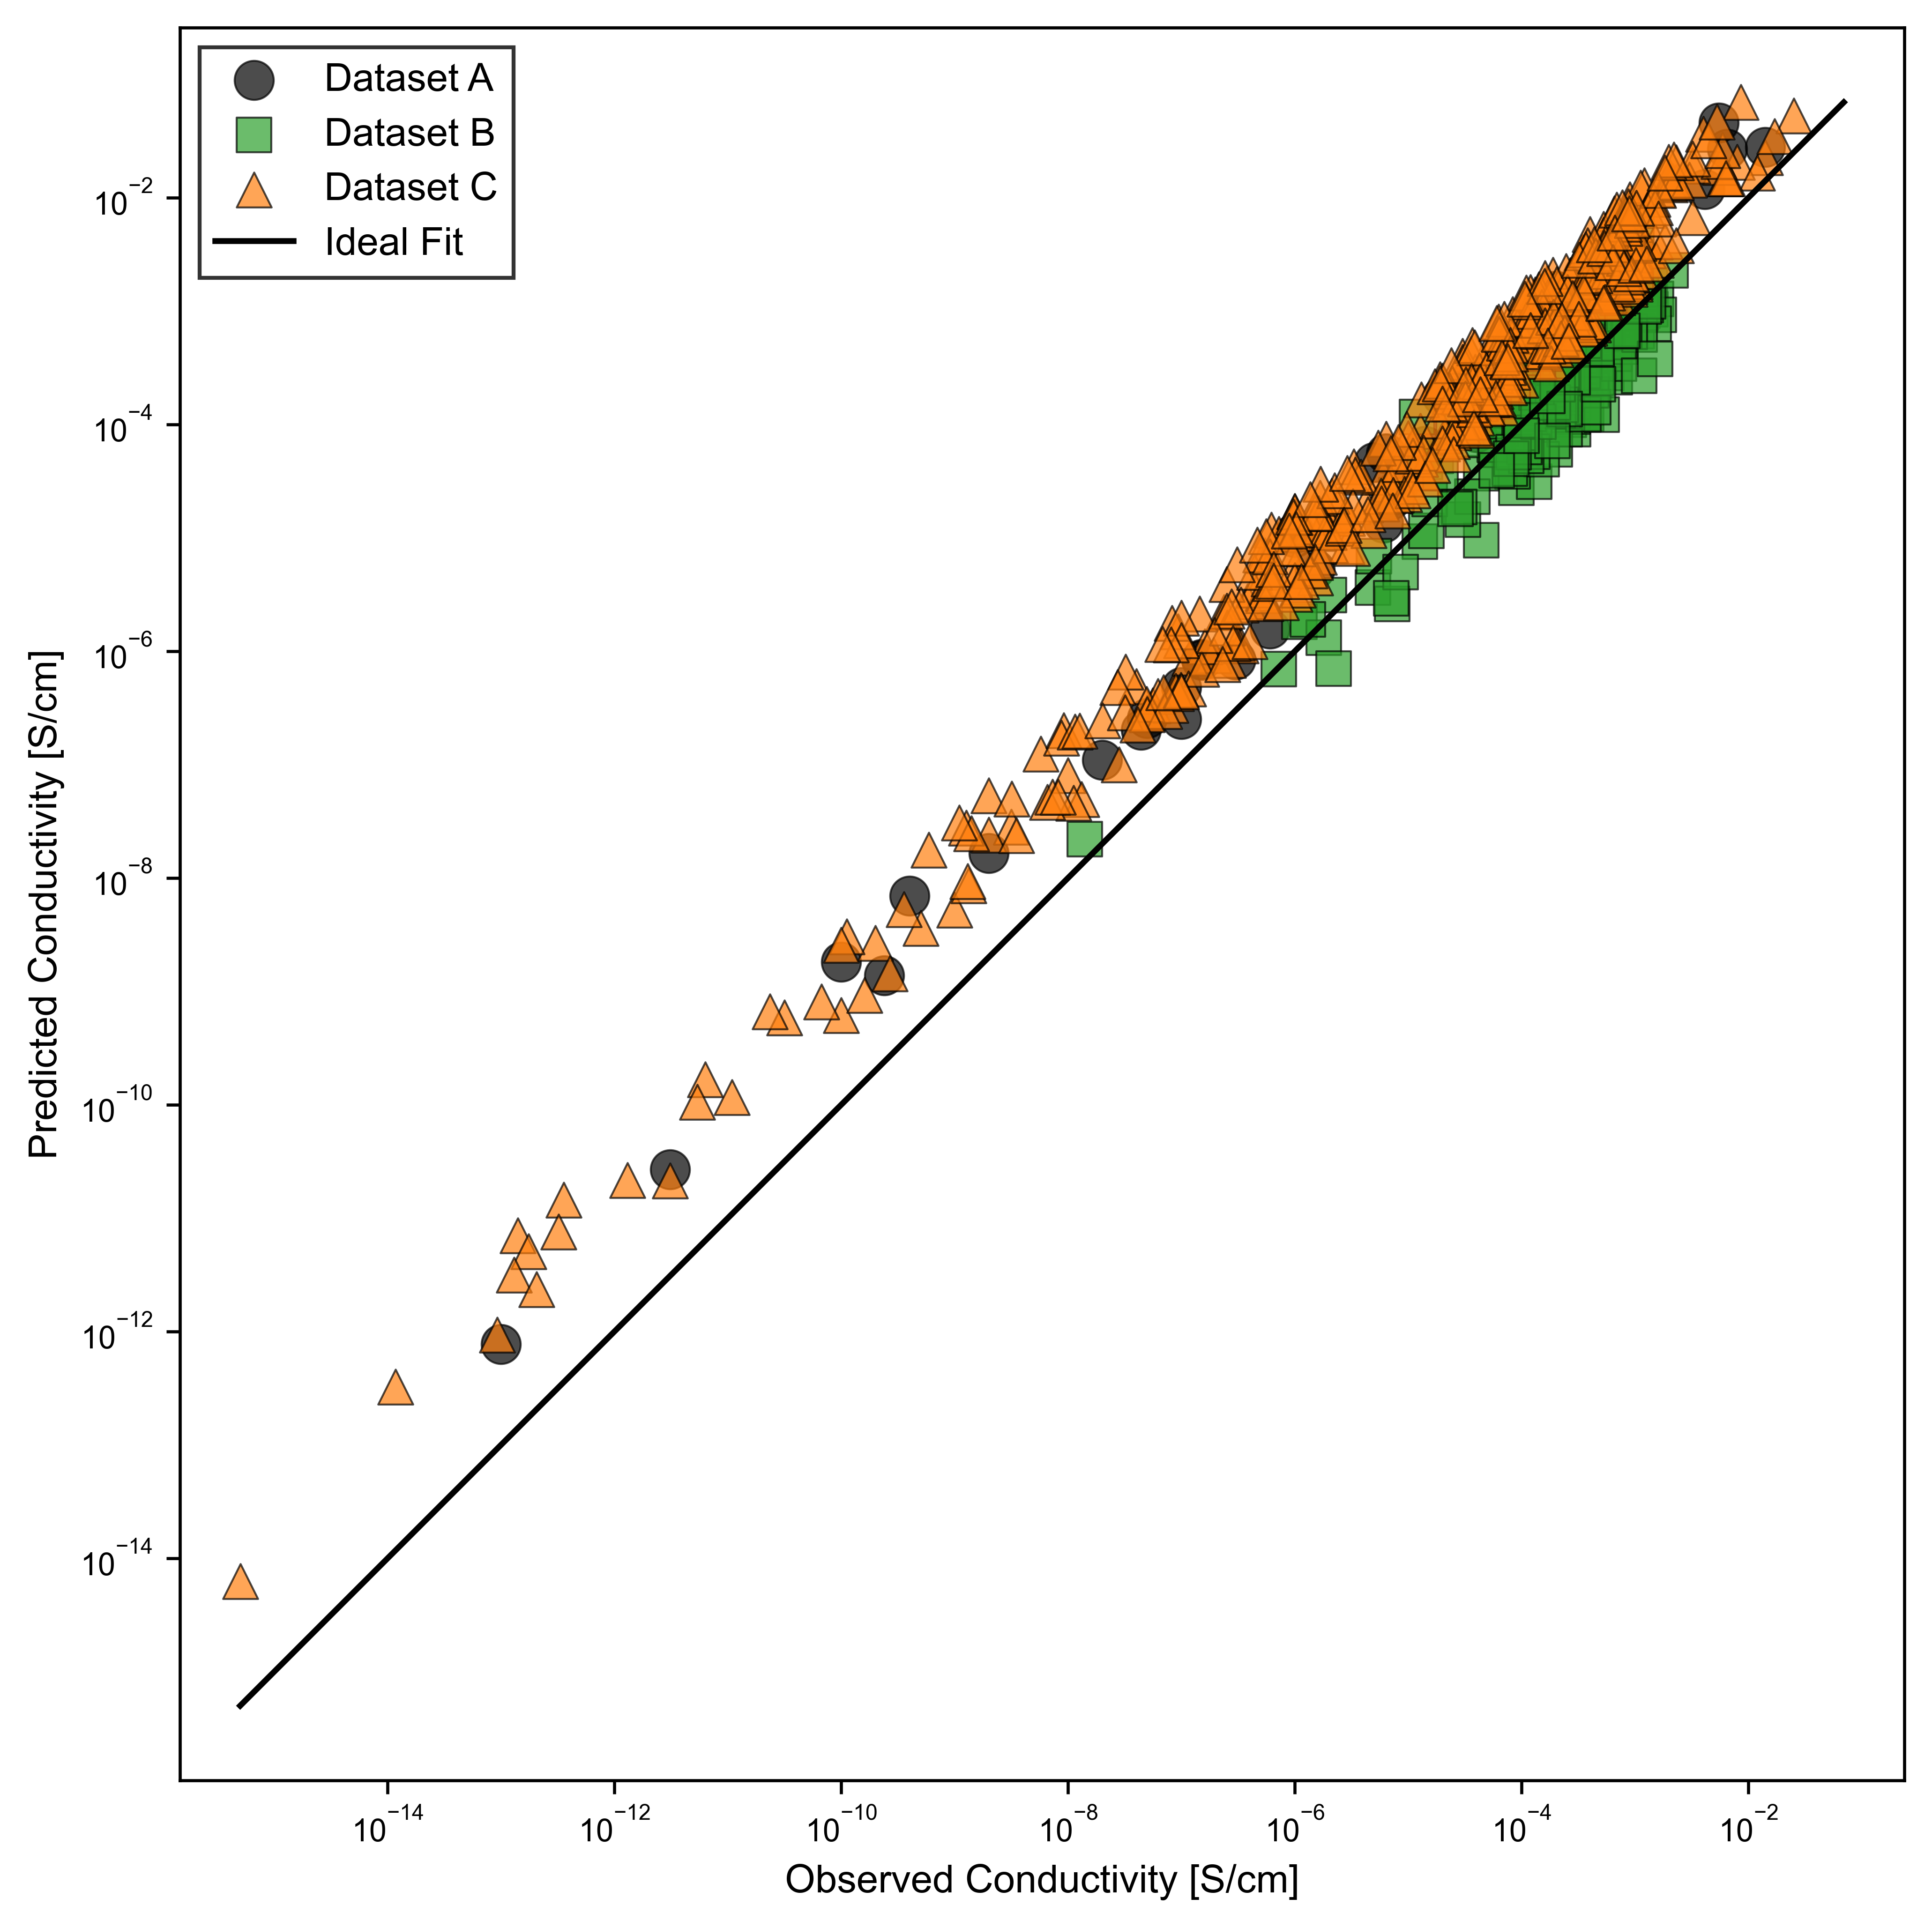
\includegraphics[width=0.6\textwidth]{Images/ddse_parity_plot.png}
\caption{Parity plot of predicted vs. observed 
$\log_{10}(\sigma)$ for the test set.}
\label{fig:ddse_parity}
\end{figure}

Furthermore, the distribution of the prediction errors was analyzed, as shown in Figure \ref{fig:ddse_error}. The histogram reveals that the errors (observed - predicted) are centered close to zero and approximate a normal distribution. This confirms that there are no severe systematic biases in the model's predictions for this dataset.

\begin{figure}[h!]
\centering
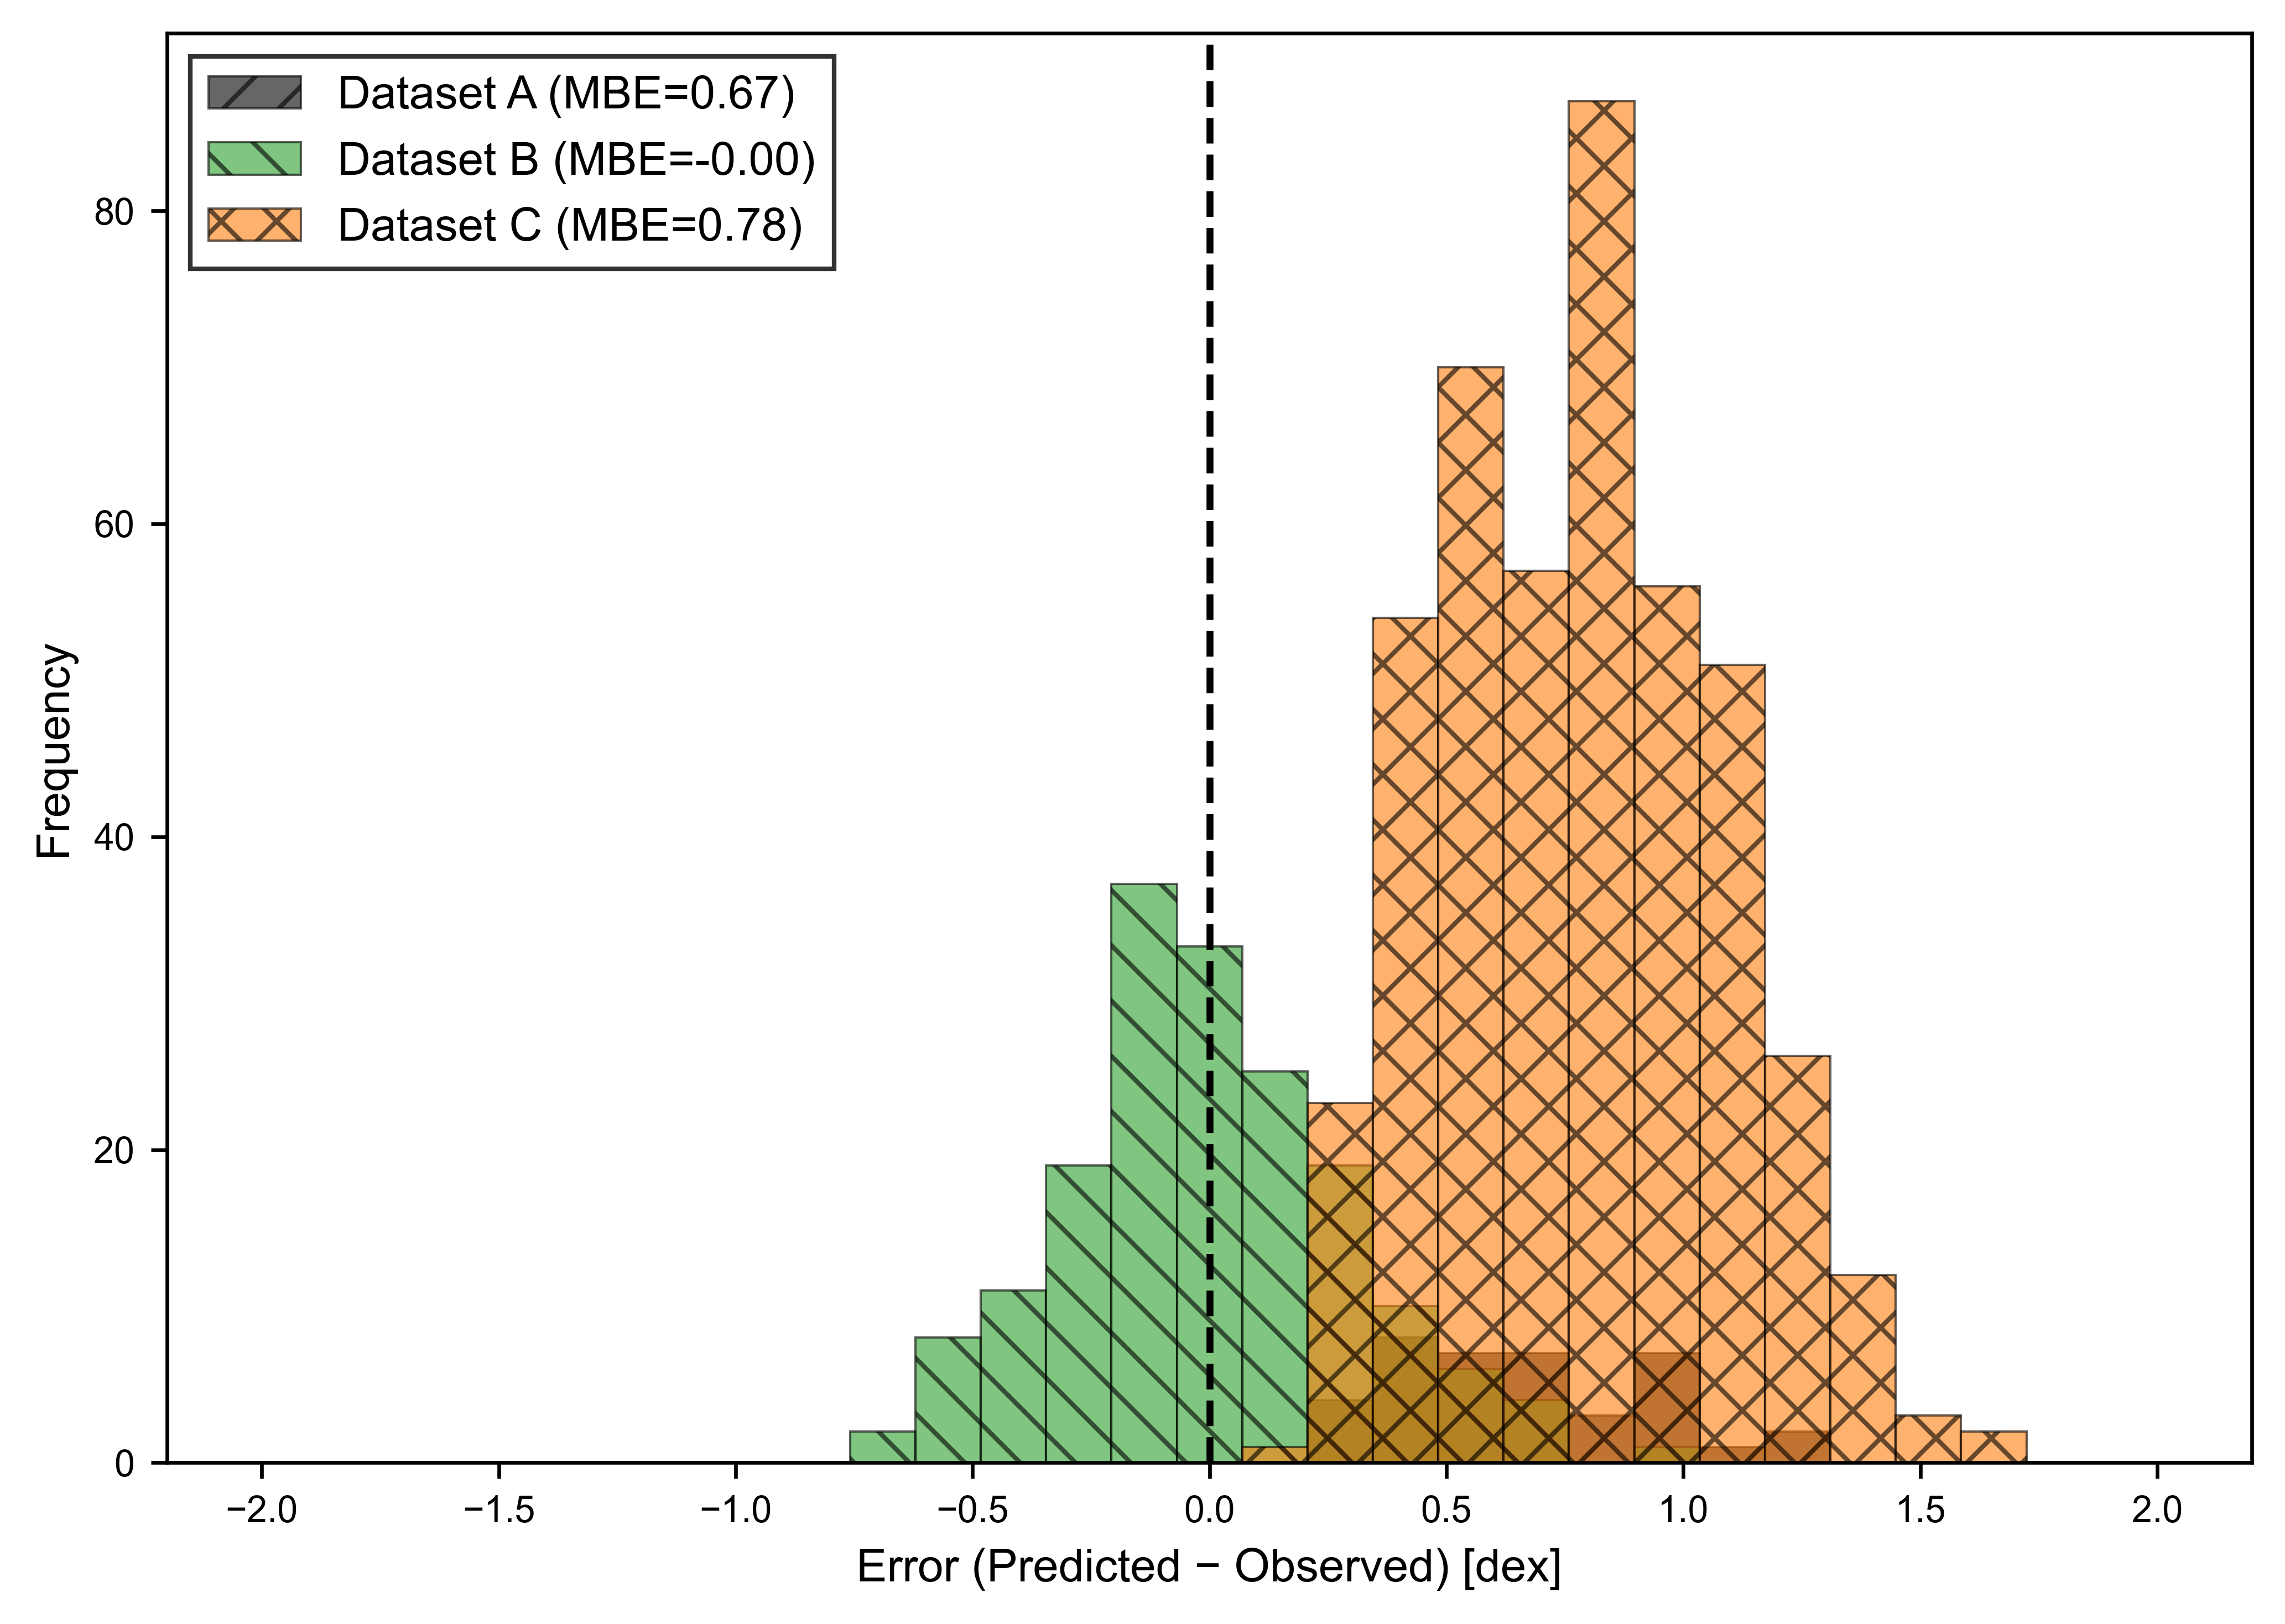
\includegraphics[width=0.6\textwidth]{Images/error_dist.png}
\caption{Histogram of the prediction errors on the DDSE test set.}
\label{fig:ddse_error}
\end{figure}

\section{External Validation on Independent Datasets}

A true test of a machine learning model's robustness and scientific value is its ability to generalize to data from different sources or chemical spaces that were not part of its original training data. To this end, we validated our trained model against three distinct external datasets compiled from the literature:
\begin{itemize}
    \item \textbf{Dataset A:} A database of Li-ion conductors compiled from literature associated with University College London \cite{Famprikis2019}.
    \item \textbf{Dataset B:} A curated dataset focusing on LLZO (Li7La3Zr2O12)-type garnet conductors \cite{Miara2015}.
    \item \textbf{Dataset C:} A well-known dataset of potential Li-ion conductors from the work of Sendek et al. \cite{Sendek2017}.
\end{itemize}

These three datasets comprise a total of 657 unique material compositions that were not present in the DDSE training set. The performance of our model on these external datasets is summarized in Table \ref{tab:external_validation}.

\begin{table}[h!]
\centering
\caption{Evaluation matrix for the trained model on different external datasets (A, B, and C) not used during training.}
\label{tab:external_validation}
\begin{tabular}{lccccccc}
\hline
\textbf{Data set} & \textbf{N} & \textbf{\(R^2_{adj}\)} & \textbf{MAE} & \textbf{RMSE} & \textbf{MBE} & \textbf{STD} \\
\hline
A                 & 442        & 0.76                  & 0.78         & 0.83          & 0.78         & 0.29         \\
B                 & 175        & 0.74                  & 0.23         & 0.29          & -0.00        & 0.30         \\
C                 & 40         & 0.82                  & 0.66         & 0.71          & 0.66         & 0.26         \\
\hline
\textbf{Overall}  & \textbf{657} & \textbf{0.78}         & \textbf{0.62} & \textbf{0.72} & \textbf{0.56} & \textbf{0.45} \\
\hline
\end{tabular}
\end{table}

The model achieved an impressive \textbf{overall adjusted \(R^2\) of 0.78} across all 657 external samples, demonstrating remarkable generalization capability. The model performs consistently well across the different chemical spaces, with a particularly strong \(R^2_{adj}\) of 0.82 on the Sendek dataset (Dataset C). This high-level performance provides powerful evidence that the model has learned genuine composition-property relationships and is a robust tool for screening new materials.

To further analyze the model's predictive behavior on these external sets, the distribution of prediction errors was examined. Figure \ref{fig:error_boxplot} presents boxplots of the absolute percentage error for each dataset. The overall Mean Absolute Percentage Error (MAPE) across all three datasets is a low 14.0\%. The median error for all datasets is consistently low, with Dataset B showing a particularly tight error distribution.

\begin{figure}[h!]
    \centering
    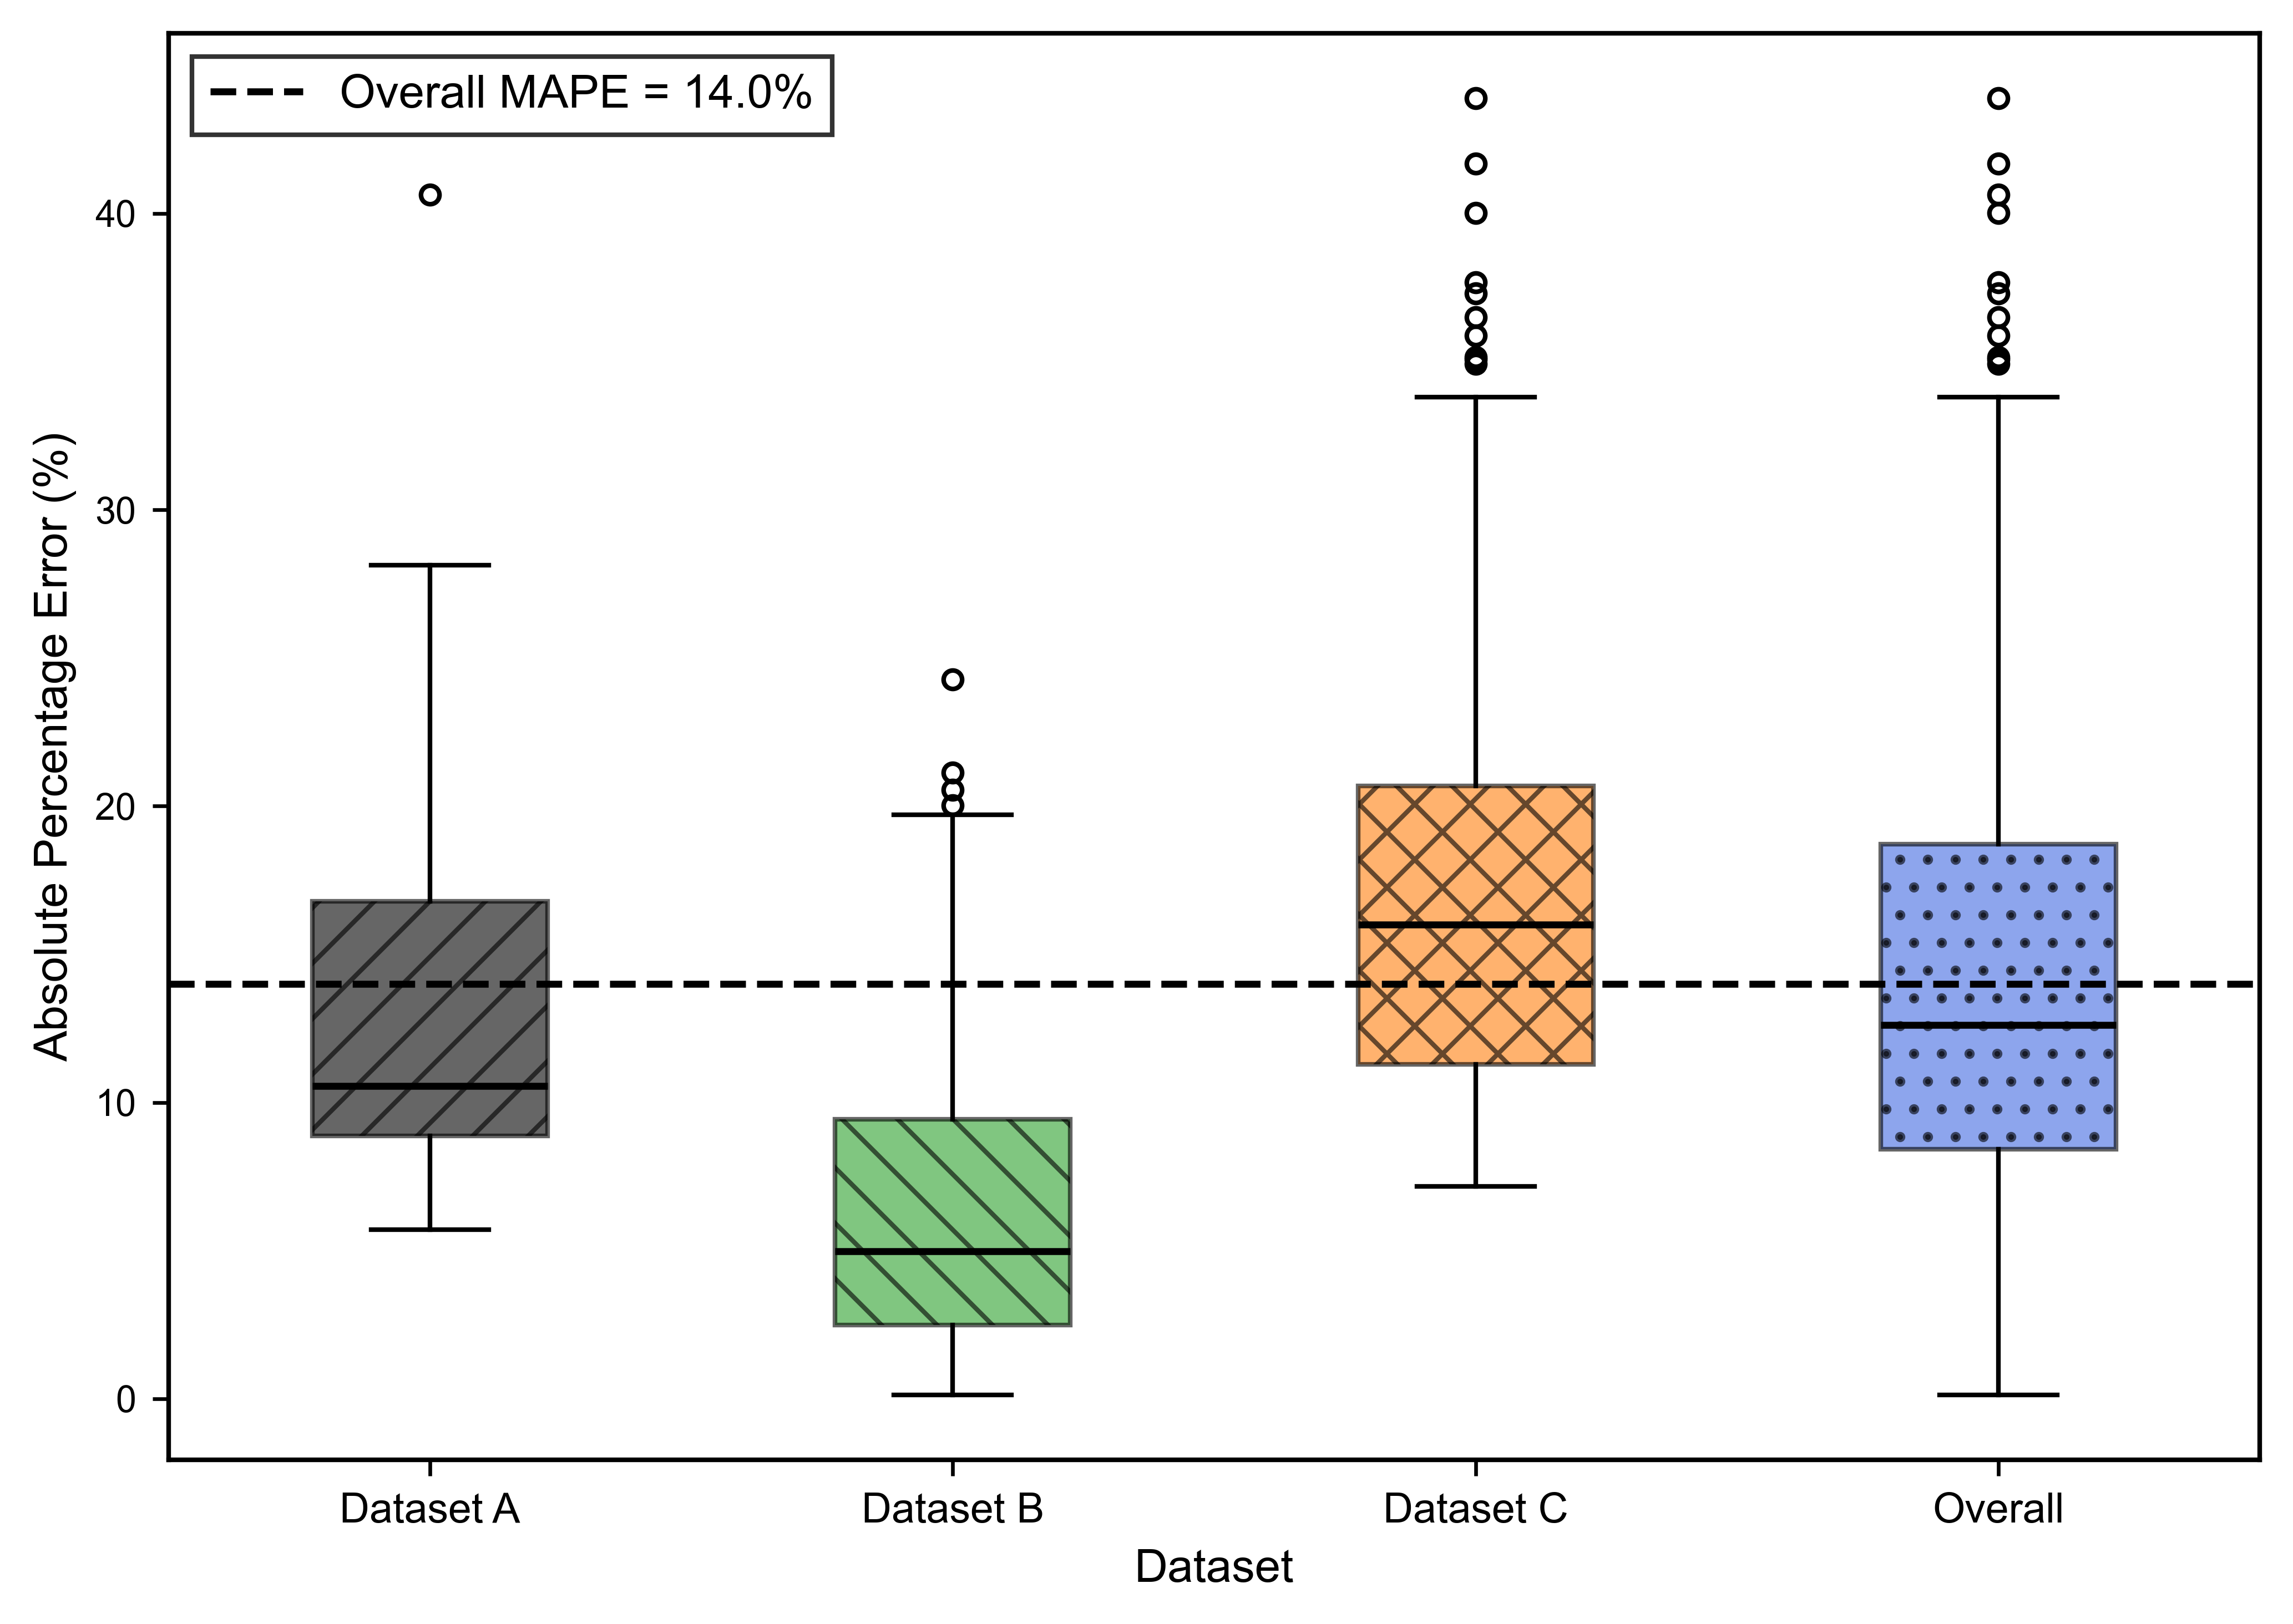
\includegraphics[width=0.8\textwidth]{Images/percent_error_box_acs.png}
    \caption{Boxplot of the absolute percentage error for each of the three external validation datasets (A, B, and C) and overall. The dashed line indicates the overall MAPE of 14.0\%.}
    \label{fig:error_boxplot}
\end{figure}

Figure \ref{fig:residuals_plot} plots the residuals (the difference between observed and predicted values, raised to the power of 10) against the observed conductivity. This plot reveals an important trend: the model's prediction error is heteroscedastic, meaning the magnitude of the error is not constant across the range of conductivity values. Specifically, the residuals are larger for materials with very low ionic conductivity (in the range of \(10^{-14}\) to \(10^{-8}\) S/cm). For materials with higher, more technologically relevant conductivities (\(>10^{-6}\) S/cm), the residuals are significantly smaller and cluster much more tightly around the zero-error line. This indicates that while the model is a strong general predictor, it is particularly accurate and reliable in the high-conductivity regime that is of greatest interest for solid-state battery applications.

\begin{figure}[h!]
    \centering
    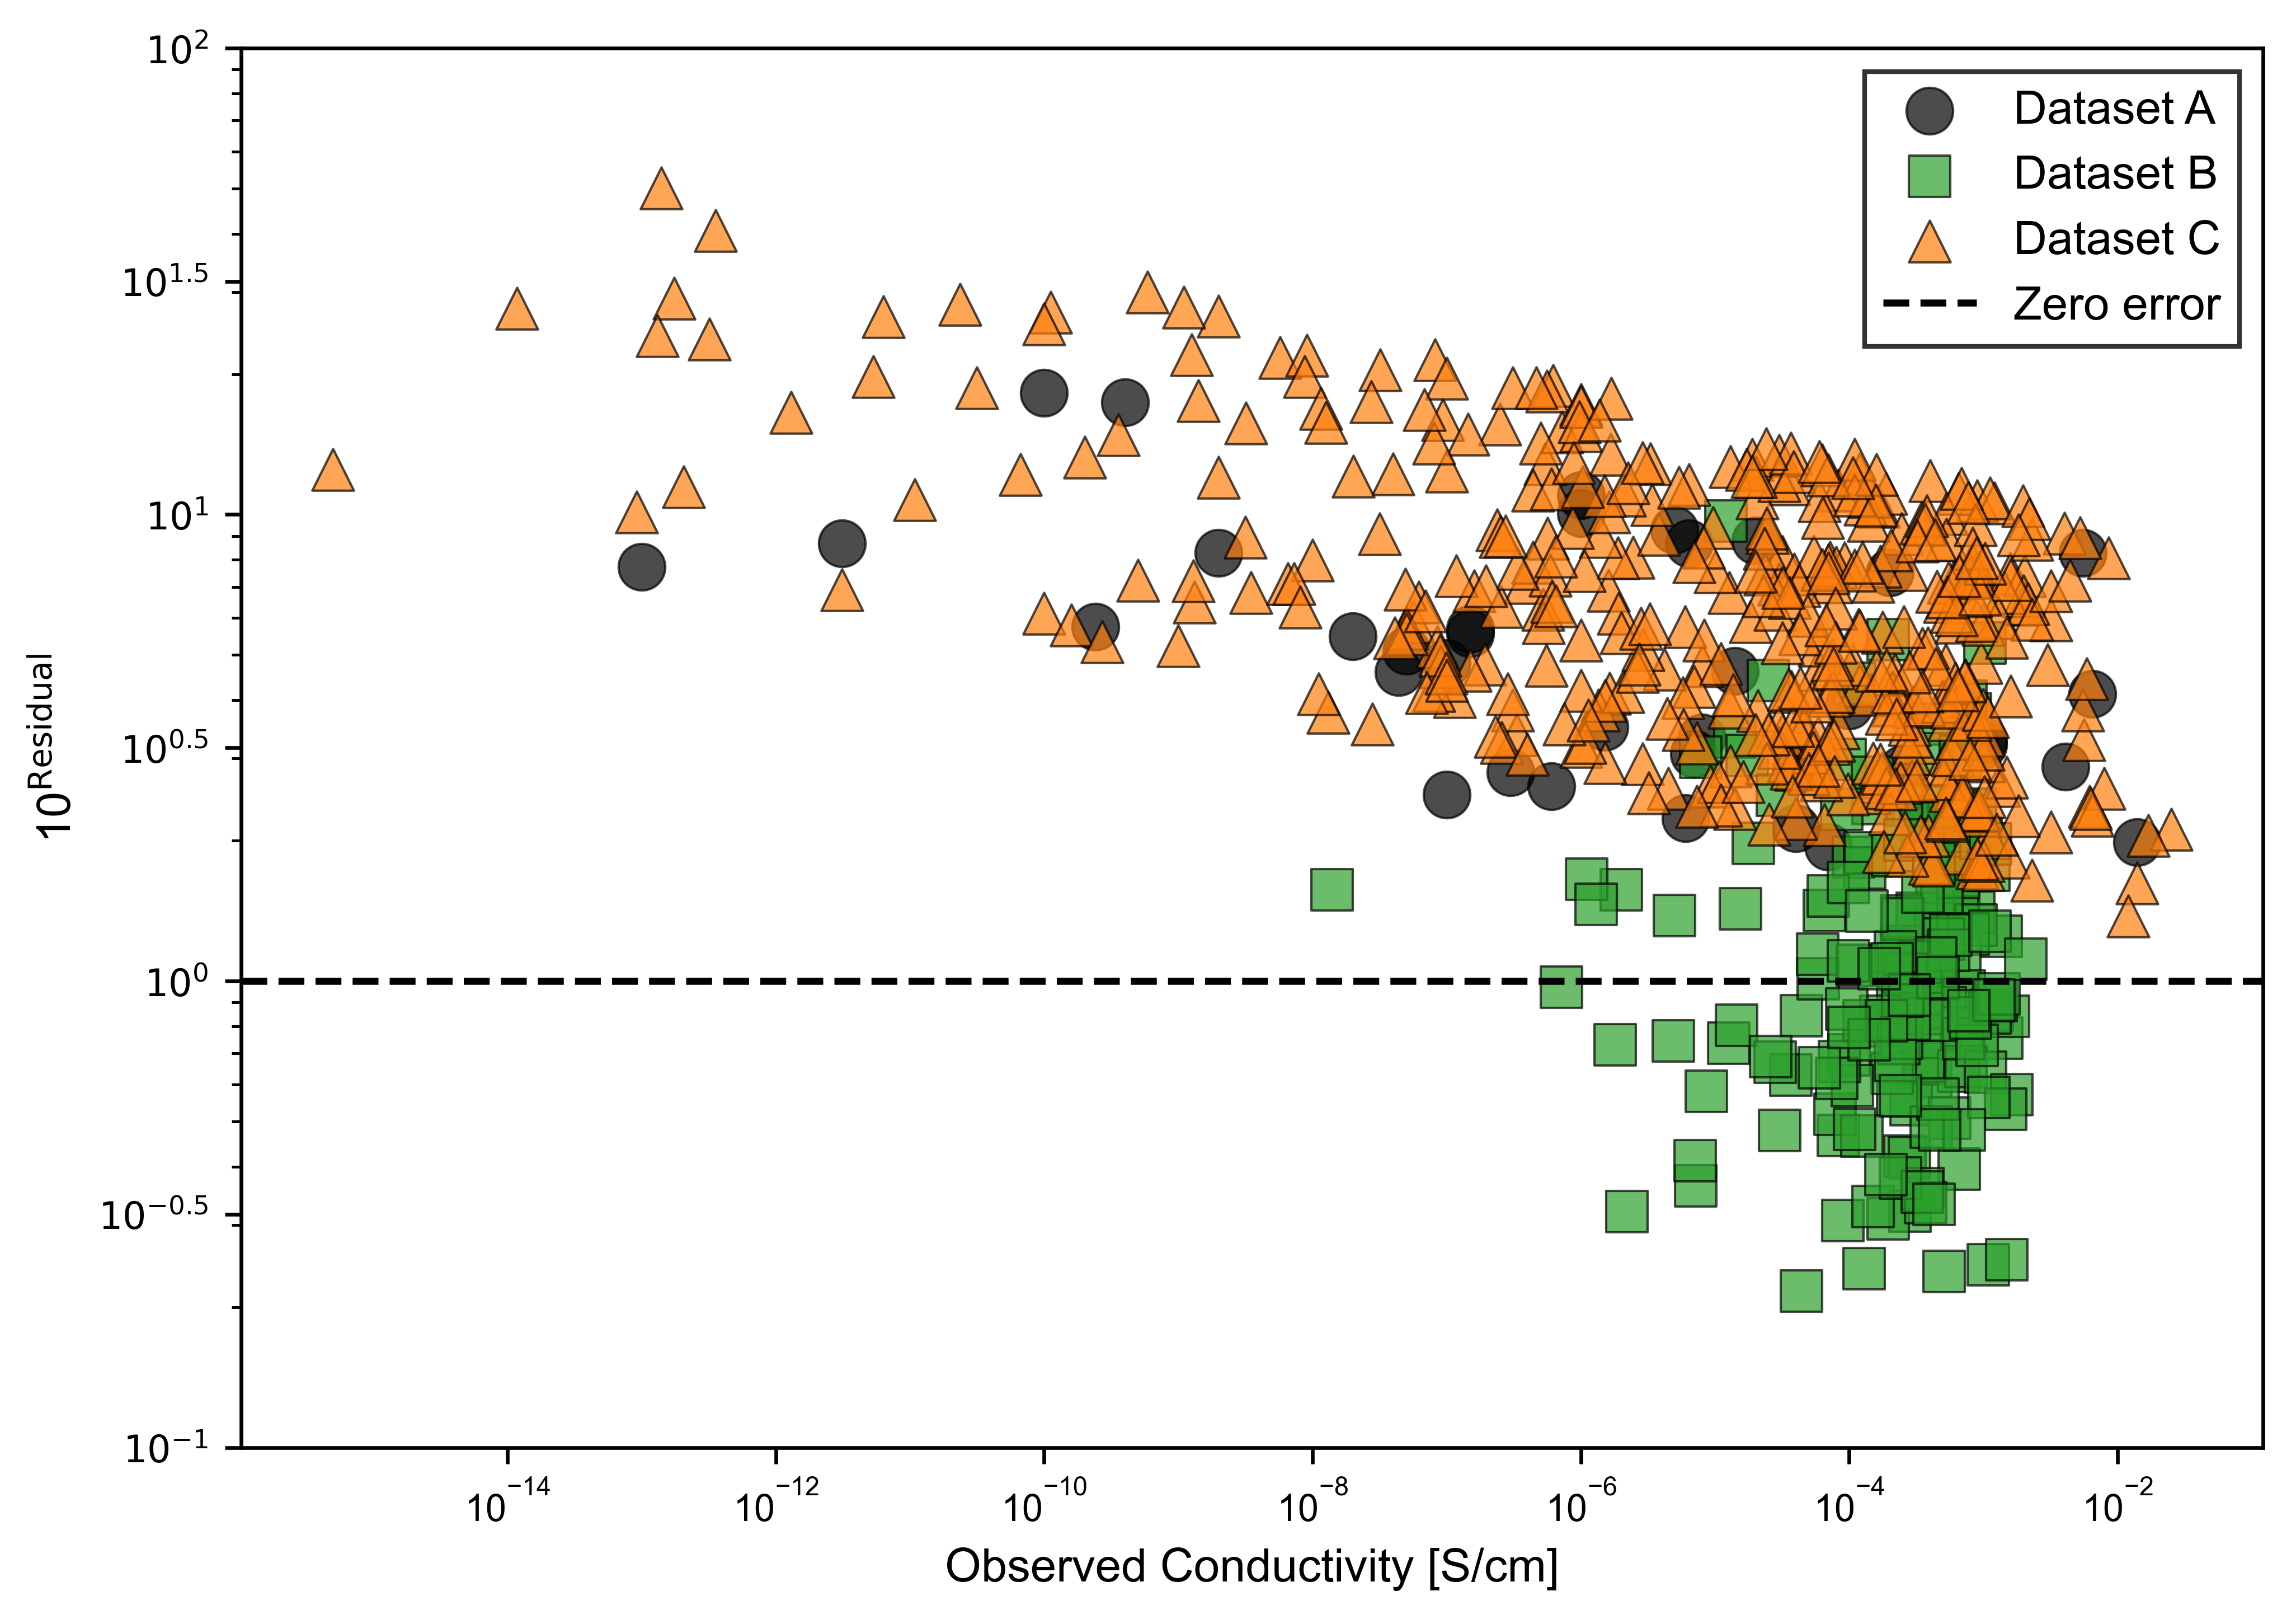
\includegraphics[width=0.8\textwidth]{Images/residuals_vs_observed_logscale_acs.png}
    \caption{Plot of the model's residuals versus the observed ionic conductivity for the external validation datasets. The plot shows that prediction errors are largest for materials with very low conductivity.}
    \label{fig:residuals_plot}
\end{figure}


% \section{External Validation on Independent Datasets}

% A true test of a machine learning model's robustness and scientific value is its ability to generalize to data from different sources or chemical spaces that were not part of its original training data. To this end, we validated our trained model against three distinct external datasets compiled from the literature:
% \begin{itemize}
%     \item \textbf{Dataset A:} A database of Li-ion conductors compiled from literature associated with University College London \cite{Famprikis2019}.
%     \item \textbf{Dataset B:} A curated dataset focusing on LLZO (Li7La3Zr2O12)-type garnet conductors \cite{Miara2015}.
%     \item \textbf{Dataset C:} A well-known dataset of potential Li-ion conductors from the work of Sendek et al. \cite{Sendek2017}.
% \end{itemize}

% These three datasets comprise a total of 657 unique material compositions that were not present in the DDSE training set. The performance of our model on these external datasets is summarized in Table \ref{tab:external_validation}.

% \begin{table}[h!]
% \centering
% \caption{Evaluation matrix for the trained model on different external datasets (A, B, and C) not used during training.}
% \label{tab:external_validation}
% \begin{tabular}{lccccccc}
% \hline
% \textbf{Data set} & \textbf{N} & \textbf{\(R^2_{adj}\)} & \textbf{MAE} & \textbf{RMSE} & \textbf{MBE} & \textbf{STD} \\
% \hline
% A                 & 442        & 0.76                  & 0.78         & 0.83          & 0.78         & 0.29         \\
% B                 & 175        & 0.74                  & 0.23         & 0.29          & -0.00        & 0.30         \\
% C                 & 40         & 0.82                  & 0.66         & 0.71          & 0.66         & 0.26         \\
% \hline
% \textbf{Overall}  & \textbf{657} & \textbf{0.78}         & \textbf{0.62} & \textbf{0.72} & \textbf{0.56} & \textbf{0.45} \\
% \hline
% \end{tabular}
% \end{table}

% The model achieved an impressive \textbf{overall \(R^2_{adj}\) of 0.78} across all 657 external samples, demonstrating remarkable generalization capability. The model performs consistently well across the different chemical spaces, with a particularly outstanding \(R^2_{adj}\) of 0.82 on the Sendek dataset (Dataset C). This high-level performance provides powerful evidence that the model has learned genuine composition-property relationships and is a robust tool for screening new materials.
